\subsection{Caratteristiche geometriche del fascio}

\begin{table}
	\centering

	\begin{tabular}{cc|cc|cc}
		\toprule
		angolo [$\si{\degree}$] & rate [$\si{s^{-1}}$] & angolo [$\si{\degree}$] & rate [$\si{s^{-1}}$] & angolo [$\si{\degree}$] & rate [$\si{s^{-1}}$] \\
		\midrule
			$-20$ & $102.8 \pm 1.1$ & $-4$ & $1310 \pm 6$  & $5$ & $544 \pm 4$       \\
			$-15$ & $149.6 \pm 1.4$ & $-3$ & $2092 \pm 8$  & $6$ & $205.5 \pm 2.1$   \\
			$-10$ & $191.4 \pm 1.7$ & $-2$ & $2847 \pm 9$  & $7$ & $173.2 \pm 1.9$   \\
			$-9$ & $208.0 \pm 1.8$  & $-1$ & $3521 \pm 11$ & $8$ & $173.7 \pm 1.6$   \\
			$-8$ & $215.2 \pm 1.8$  & $0$ & $3792 \pm 11$  & $9$ & $174.7 \pm 1.6$   \\
			$-7$ & $228.3 \pm 2.2$  & $1$ & $3426 \pm 10$  & $10$ & $170.2 \pm 1.6$  \\
			$-6$ & $298 \pm 3$      & $2$ & $2695 \pm 9$   & $15$ & $118.5 \pm 1.2$  \\
			$-5$ & $680 \pm 5$      & $3$ & $1930 \pm 8$   & $20$ & $78.4 \pm 0.9$   \\
			     &                  & $4$ & $1160 \pm 6$   &      &\\
		 \bottomrule
	\end{tabular}

	\caption{Rate senza coincidenza nei canali dell'ADC 5500--8040
	al variare dell'angolo del PMT2.
	L'errore sugli angoli è 0.1$^{\circ}$.
	Il fondo costante misurato è \SI{4.43\pm0.2}{s^{-1}}.}
	\label{tabfo}
\end{table}

\begin{figure}
	\centering
	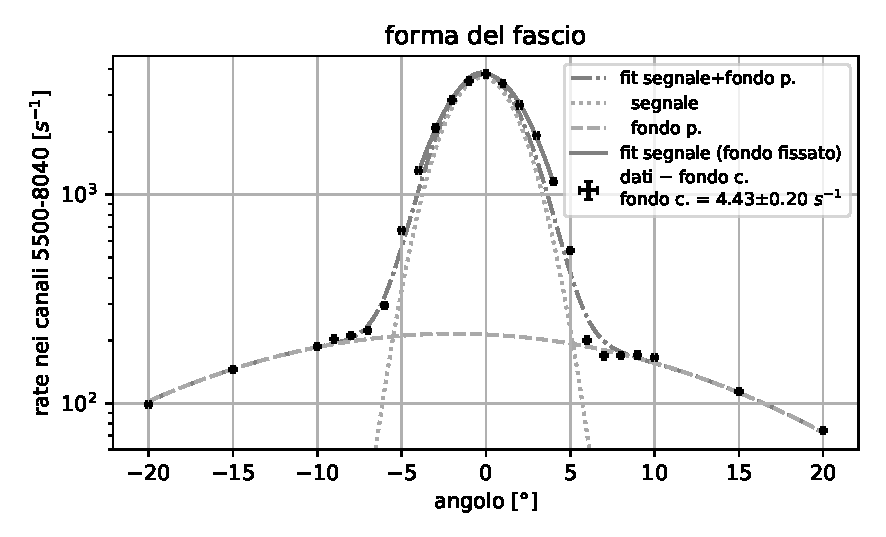
\includegraphics[width=32em]{forma}
	\caption{Dati e fit della forma del fascio.
	Nella legenda, <<fondo p.>> sta per <<fondo piccato>> e <<fondo c.>> per <<fondo costante>>.}
	\label{forma}
\end{figure}

\subsubsection{Accorgimenti sperimentali}

Ci interessa misurare la divergenza angolare del fascio.
Per farlo posizioniamo il PMT2 di fronte alla sorgente a vari angoli e triggeriamo sul PMT2 stesso. Lo scopo è disegnare un grafico dei rate in funzione dell'angolo.

Per conoscere il tempo di acquisizione montiamo un circuito che, usando un timer,
fa partire e fermare simultaneamente il trigger e il contatore.

Per misurare meglio gli angoli abbiamo stampato un goniometro che abbiamo posizionato sotto il supporto trasparente della guida su cui scorre il PMT2. Infine abbiamo tracciato un segmento sulla parte trasparente che ci permette di capire a quale angolo posizioniamo il PMT2.
Lo zero degli angoli è riferito al goniometro e otterremo il centro del fascio dalle misure.

\subsubsection{Analisi dei dati e risultati}

Scegliamo di misurare il rate solo in un intervallo di energia che contiene i due fotopicchi,
per evitare di includere eventuali fondi di raggi $\gamma$ che non provengono direttamente dalla sorgente.
L'intervallo è abbastanza largo che il piccolo spostamento dei fotopicchi al variare dell'angolo del PMT2 non fa intersecare i fotopicchi con i bordi.
Facciamo anche una misura di <<fondo costante>> con il PMT2 posizionato in un punto non visibile dalla sorgente,
ma con la sorgente aperta.

Le misure sono riportate in \autoref{tabfo}.
La misura di fondo costante risulta praticamente trascurabile.
In \autoref{forma} sono riportati i dati con sottratto il fondo costante.
Si nota che la forma sembra essere la somma di due gaussiane (che sono parabole in scala logaritmica).
Chiamiamo la gaussiana più larga <<fondo piccato>>
e la interpretiamo come raggi che non provengono direttamente dalla sorgente
perché si nota un'asimmetria rispetto al centro, che non c'è nella gaussiana stretta (il <<segnale>>)
e che non corrisponde alla geometria cilindrica del collimatore.

Se fittiamo una gaussiana per i dati dagli angoli \SI{-5}\degree{} a \SI5\degree{} otteniamo già un buon accordo.
Tuttavia, vista la nostra interpretazione, riteniamo più sensato sottrarre il fondo piccato.
A causa dell'asimmetria del fondo, se fittiamo le due gaussiane non otteniamo un buon accordo
e la gaussiana di segnale viene fittata visibilmente peggio.
In sostanza: sappiamo modellare bene il segnale ma non il fondo.
Allora estraiamo il fondo dal fit delle due gaussiane,
lo sottraiamo e fittiamo la sola gaussiana di segnale da \SI{-4}\degree{} a \SI4\degree.

La deviazione standard del segnale risulta \SI{2.52 \pm 0.03}{\degree},
il centro \SI{-0.09 \pm 0.04}{\degree}.
Dal segnale dobbiamo deconvolvere la forma dello scintillatore NaI,
la cui deviazione standard è \SI{1.82 \pm 0.07}\degree, ottenuta sapendo che è un cilindro di raggio \SI{2}{''}
e che dista \SI{40\pm 1.5}{cm} (l'incertezza sulla distanza è data dalla profondità dello scintillatore e dalla larghezza del collimatore).
La deviazione standard della forma del fascio si ottiene semplicemente dalla sottrazione in quadratura
e risulta \SI{1.73 \pm 0.09}{\degree}.
